\documentclass[11pt, english, fleqn, DIV=15, headinclude, BCOR=2cm]{scrreprt}

\usepackage[
    color,
    bibatend,
]{../../header}

\graphicspath{{_build/}{../Figures/}}

\hypersetup{
    pdftitle=
}

\usepackage{longtable}

\newcommand\tRL{t_\text{RL}}
\newcommand\tLR{t_\text{LR}}
\newcommand\nRL{n_\text{RL}}
\newcommand\nLR{n_\text{LR}}
\newcommand\vRL{v_\text{RL}}
\newcommand\vLR{v_\text{LR}}
\newcommand\rateRL{\dot n_\text{RL}}
\newcommand\rateLR{\dot n_\text{LR}}

\subject{Lab report}
\title{Mößbauer effect}
\subtitle{Experiment K221 -- Universität Bonn}
\author{%
    Martin Ueding \\
    \small{\href{mailto:mu@martin-ueding.de}{mu@martin-ueding.de}}
    \and
    Lino Lemmer \\
    \small{\href{mailto:l2@uni-bonn.de}{l2@uni-bonn.de}}
}

\date{2016-03-02}

\publishers{Tutor: Peter Klassen}

\begin{document}

\maketitle

\begin{abstract}
    In this experiment we examine the $\gammaup$-spectrum of
    $^{57}\mathrm{Fe}$. The aim is to find the Landé factors $g$ for the ground
    state and the first excited state by measuring the hyperfine structure and
    Mößbauer spectrum respectively of the $\SI{14.4}{\kilo\electronvolt}$
    transition. Line widths and the isometric shift are to be determined from
    the spectrum. By this a deeper understanding of recoilless emission and
    absorption as well of basic terms in nuclear physics should be achieved.
\end{abstract}

\tableofcontents

\chapter*{Permission to upload}

I, Martin Ueding, would like to scan and upload this lab report with your
corrections to my website \href{http://martin-ueding.de}{martin-ueding.de}.
There, the original lab report as well as the reviewed one will be licensed
under the “\href{http://creativecommons.org/licenses/by-sa/4.0/}{Creative
Commons Attribution-ShareAlike 4.0 International License}”. Is that okay with
you?

Yes $\Box$ \hspace{2cm} No $\Box$

\chapter{Theory}

\section{Absorption and resonances}

Like the electrons in an atom, the constituents of a nucleus also have
excited states and associated energy levels. As the nucleus is orders of
magnitude smaller than the whole atom, the relevant energies are orders of
magnitude larger. The hydrogen transition energies are in the order of
\SIrange{1}{10}{\electronvolt} whereas the transition energies cobalt and iron
are in the order of \SIrange{10}{100}{\kilo\electronvolt}.

If the energy matches an allowed transition, a nucleus can also absorb
electromagnetic radiation and transition into an excited state. As most nuclei
in a metal are in the groundstate, the highest absorption can be obtained by a
transition from the groundstate. Photons with the required energy are created
by an excited nucleus of the same isotope decaying into the groundstate.

The experimental setup here has a radiation source made from cobalt
($^{57}\text{Co}$). This decays into excited iron ($^{57}\text{Fe}$) via
electron capture (EC), see Figure~\ref{fig:ec}. The excited nucleus in turn
will decay into the groundstate via some metastable states. See
Figure~\ref{fig:co57} for the decay scheme of the radioactive material used in
this experiment. The transition into the groundstate is the one from $j^P =
3/2^-$ to $1/2^-$ with an energy gap of $\hbar \omega_0 =
\SI{14.4}{\kilo\electronvolt}$.

\begin{figure}
    \centering
    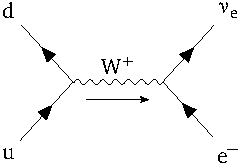
\includegraphics{ec}
    \caption{%
        Electron capture, leading order contribution. Time goes upwards.
    }
    \label{fig:ec}
\end{figure}

\begin{figure}
    \centering
    \includegraphics{co57}
    \caption{%
        Decay scheme of $^{57}\mathrm{Co}$ into $^{57}\mathrm{Fe}$. Cobalt from
        the source undergoes electron capture (EC) with a very long halftime.
        The transition between to the groundstate (thick) is the Mößbauer
        energy level we are interested in.
        %
        Figure adapted from
        \textcite[Fig.~4.8]{Schatz/Nukleare_Festkoerperphysik}.
    }
    \label{fig:co57}
\end{figure}

The emission lines are not perfectly sharp. This limits the chance of
absorption by the same kind of nucleus. The broadening effects are the
following:

\begin{description}
    \item[Natural width]
        The lifetime $\tau$ of every metastable state is limited. If it were
        not, one would not observe the transition. Together with the
        energy-time-uncertainty this directly leads to a line width of
        \[
            \Gamma = \frac\hbar\tau \,.
        \]
        This broadening via finite lifetime leads to an Lorentzian line shape
        stemming from the Breit-Wigner prescription for a resonance which is a
        good approximation for narrow resonances.

        Our line of interest, the \SI{14.4}{\kilo\electronvolt}-line, has a
        lifetime of \SI{141}{\nano\second} and therefore a width of $\Gamma =
        \SI{4.7e-9}{\electronvolt}$. Compared to energy of the photons
        themselves, this is a relative width of \num{3.3e-13}. That is very
        small compared to the other effects.
        \parencite[42]{Schatz/Nukleare_Festkoerperphysik}

    \item[Doppler effect]
        A relative motion between source and target will lead to a Doppler
        shift. The Lorentz transformation connecting the two systems boosts the
        photon's energy. Linearizing the $\cosh(\rho)$, we obtain a boosted
        energy of $\hbar\omega_0(1 + v/c)$. If the source particles are subject
        to thermal motions, the spectrum will be broadened. At room
        temperature, the shifts in energy are around \SI{10e-2}{\electronvolt}
        \parencite[43]{Schatz/Nukleare_Festkoerperphysik}, depending on the
        angle of motion and emission. Doppler broadening leads to an Gaussian
        line shape.

        The natural line width can be ignored when the thermal Doppler effect
        is present.

    \item[Recoil]
        The photon carries momentum $\hbar k$. In the center of mass frame of
        the emitting nucleus, the nucleus will take the recoil $- \hbar k$. The
        energy of the nucleus then is $(\hbar k)^2/2 M$, where $M$ is the mass
        of nucleus. This energy is subtracted from the photon; the photon has a
        reduced frequency when emitted from a free nucleus.
\end{description}

Taking all those effects together, it becomes unlikely that the photons emitted
by a gas of decaying cobalt will be absorbed by a gas of iron, ignoring that it
might be impractical to realize this situation experimentally. The issue of the
recoil can be reduced by embedding the nuclei of interest into a solid state.
The lattice will absorb the excess momentum and due to its practically infinite
mass (some \num{e23} larger), there will be no recoil velocity and therefore no
energy shift in the photon.

\section{Debye-Waller Factor}

Although there is no energy shift caused by recoil, the energy is still shifted
due to thermal motion of the atoms. Even at $T = \SI{0}{\kelvin}$, there will
be a shift because of zero-point energy. To get a measure of how temperature,
$\gammaup$-energy and mass of the lattice influence the emission, one can find
the Debye-Waller factor, which is the ratio of the unshifted spectrum to the
real one. For temperatures below the material specific Debye
temperature~$\Theta$, the factor is given by
\[
    f_\text{D} (T, E_\gammaup, M)
    = \exp \del{
        - \frac{3E_\gammaup^2}{4Mc^2k_\text{B}\Theta}
        \sbr{1 + \frac{2\piup^2}3 \del{\frac T\Theta}^2}
    } \,,
\]
analog to the expression given by
\textcite[42]{Schatz/Nukleare_Festkoerperphysik}.

For iron, the Debye temperature is $\Theta = \SI{470}{\kelvin}$
\parencite[Tab.~6.1]{Hunklinger/Festkoerperphysik}, so we are well below this
in our experiment. Together with $E_\gammaup = \SI{14.4}{\kilo\electronvolt}$,
the iron mass $M = \SI{<< iron_mass >>}{\kilogram}$ and assuming room
temperature ($T = \SI{<< room_temp >>}{\kelvin}$), we see that the fraction has
the value \num{<< debye_1 >>}, the square bracket has the value \num{<< debye_2
>>} which yields a total Debye-Waller factor of \num{<< debye_3 >>} for our
experimental situation. This is high enough to give a decent signal-to-noise
ratio.

\section{Magnetic hyperfine structure}

The angular momentum~$l$ and the spin~$s$ of the nucleus couple to a combined
spin~$j$. The component along the quantization axis, $m_j$, takes values
between $-j$ and $j$. The various states organize themselves into the
irreducible representations of $\SU(2)$, the multiplets with spin~$j$ and
$(2j+1)$ states each. The different multiplets have different energies, the
energies within the same multiplet are degenerate, see left part of
Figure~\ref{fig:M1}. Breaking the $\SU(2)$ symmetry of the spins give the
nuclear analogue of the Zeeman effect. This is done with an external magnetic
field by the interaction term $- \vec\mu \cdot \vec B$. The degeneracy is
broken and each multiplet is split up into equidistant levels, see the right
part of said figure.

The magnetic moment~$\vec \mu$ is related to the spin~$j$ via the nuclear
magneton~$\mu_\text N$ or the gyromagnetic ratio~$\gamma$,
\[
    \mu = \underbrace{g \frac{\mu_\text N}{\hbar}}_{\gamma} \hbar j \,.
\]
Choosing the quantization axis along the external magnetic field $\vec B$ will
simplify the interaction $- \vec \mu \cdot \vec B$ to $- |\vec B| g \mu_\text N
m_j$. The $m_j$ are (half-)integers and therefore equidistant. This makes the
energy levels equidistant within a multiplet.

\begin{figure}
    \centering
    \includegraphics{M1}
    \caption{%
        Hyperfine structure of the \SI{14.4}{\kilo\electronvolt}-M1-line in
        $^{57}\mathrm{Fe}$, our Mößbauer transition.
        Figure adapted from
        \textcite[Fig.~4.22]{Schatz/Nukleare_Festkoerperphysik}.
    }
    \label{fig:M1}
\end{figure}

Both source and target are embedded into a solid, therefore there is little
thermal fluctuation and also very little recoil. This means that the lines are
rather sharp. Only the target nuclei is embedded into a magnetic field. This
magnetic field comes from the magnetic domains in the ferromagnetic iron metal.
The source iron nuclei do not have the Zeeman splitting and therefore always
emit a pretty exact \SI{14.4}{\kilo\electronvolt} line. In order for the target
in the magnetic field to absorb the emitted photons, their energy needs to be
adjusted.

By moving the target with a motor, one can leverage the Doppler shift to alter
the energy of the photon. As this velocity is controlled, one can effectively
measure the energy shifts and therefore the hyperfine structure in the iron
target. We are interested in the deviation from $\hbar \omega_0 =
\SI{14.4}{\kilo\electronvolt}$ and want to extract the magnetic moment of the
groundstate and the exited state.

The needed relation between Doppler velocity $v$ and the magnetic moments
$\mu$, $\mu'$ is
\[
    v = \frac{c B}{\hbar \omega_0}
    \sbr{\frac{\mu}{j} m_j - \frac{\mu'}{j'} m_j'}
    \,,
\]
where the primed quantities are the exited state
\parencite[(4.42)]{Schatz/Nukleare_Festkoerperphysik}. Expressing the magnetic
moments in terms of the nuclear magneton, we see the relation between the Landé
factors more clearly:
\begin{equation}
    \label{eq:velocity}
    v = \frac{c B \mu_\text N}{\hbar \omega_0} \sbr{g m_j - g' m_j'} \,.
\end{equation}
Inside the solid, the magnetic flux density is \SI{<< B >>}{\tesla}. All other
quantities are known,
the prefactor has the value \SI{<< v_prefactor >>}{\meter\per\second}. As $g$
and $m_j$ are of the order of magnitude one, the experimental setup with
$v_\text{max} = \SI{0.006}{\meter\per\second}$ will be sensible.

The selection rule for magnetic dipole (M1) radiation is $(m_j - m_j') \in \{
-1, 0, 1 \}$. Therefore we expect to see six velocities with high absorption.

\section{Isomeric shift and quadrupole moment}

The iron nuclei in the source and target are embedded into a solid. This means
that each nucleus is surrounded by a lot of other charged particles which
create a non-constant electric field. The nucleus is not a point charge,
therefore it does interact with the electric potential beyond a monopole
interaction.

We assume that the electric potential that is created outside of the nucleus
does not vary too much across the volume of the nucleus. Then we can expand the
electric potential around the nucleus like
\[
    \Phi(\vec r) = \Phi_0 + \pd{\Phi}{x^i} x^i
    + \frac12 \frac{\partial^2 \Phi}{\partial x^i \partial x^j} x^i x^j +
    \mathrm O(x^3) \,,
\]
where we have used Einstein's summation convention
\parencite[(3.19)]{Schatz/Nukleare_Festkoerperphysik}. We can identify three
terms:

\begin{description}
    \item[Constant]
        The constant term is the monopole interaction, it just gives rise to a
        common shift in the energies and is not relevant for our experiment as
        we can only observe the difference in energy levels, i.e.\ the photon
        energy.

    \item[Linear]
        The gradient is a dipole interaction. Quantum mechanics enforces the
        nuclear states to be parity eigenstates, therefore the expectation
        value of the dipole moment is zero. The linear term does not create any
        shift in the energy.

    \item[Quadratic]
        The Hessian gives rise to an electric quadrupole interaction and the
        isomeric shift. We will need to further analyze the Hessian.
\end{description}

The shift in energy by each of those terms is given by an appropriate
integration against the charge density of the nucleus. For the quadratic term
we have
\[
    E^{(2)} = \frac 12 \frac{\partial^2 \Phi}{\partial x^i \partial x^j}
    \int \dif^3 r \, \rho(\vec r) \, x^i x^j \,.
\]
Since the Hessian is a real symmetric matrix, it can be diagonalized by an
orthogonal transformation. Let the eigenvalues of the Hessian be $\lambda_i$,
then we can split up the electric energy like follows into a pure-trace and a
traceless term:
\begin{align*}
    E^{(2)}
    &= \frac12 \sum_i \lambda_i \int \dif^3 r \, \rho(\vec r) \, x_i^2 \\
    &= \frac16 \sum_i \lambda_i \int \dif^3 r \, \rho(\vec r) \, r^2
    + \frac12 \int \dif^3 r \, \rho(\vec r) \sum_i \lambda_i \sbr{x_i^2 -
    \frac{r^2}3} \,.
\end{align*}
The electric potential also obeys the Poisson equation, therefore we also have
\[
    \laplace \Phi = \sum_i \lambda_i = \frac{e}{\varepsilon_0} |\psi(0)|^2 \,,
\]
i.e.\ the charge density at the origin by the electron wave functions is
proportional to the trace of the Hessian. The first summand in the above
splitting is the isomeric term and we can rewrite it as
\[
    E_\text I := \frac16 \frac{e}{\varepsilon_0} |\psi(0)|^2
    \int \dif^3 r \, \rho(\vec r) \, r^2 \,.
\]
The integral over the charge density with $r^2$ is the second moment of the
charge distribution and therefore proportional to $\bracket{r^2}$, the
expectation value of the squared radius. The proper normalization includes
$1/Ze$.

We see that the isomeric term depends on the shape of the nucleus but does not
lead to any splitting depending on $m_j$ like we saw with an external magnetic
field.
The energy difference can be expressed as a Doppler velocity
\[
    v = \frac{Z e^2 c}{6 \varepsilon_0 \hbar \omega_0}
    \del{|\psi_\text T(0)|^2 - |\psi_\text S(0)|^2}
    \del{\bracket{r^2_\text{e}} - \bracket{r^2_\text{g}}} \,,
\]
as given by \textcite[(4.31)]{Schatz/Nukleare_Festkoerperphysik}. If the iron
nuclei in source (S) and target (T) are embedded into different crystals, then
$|\psi(0)|^2$ will be different there. We also need the mean squared radius of
the excited (e) and ground (g) state to differ in order for this effect to be
picked up. In our experiment we will see this as a common shift independent of
$m_j$.

The second term in the splitting is the quadrupole term. If the potential is
$\SO(3)$ symmetric, all the eigenvalues~$\lambda_i$ are equal. The three
summands will all yield the same term, the sum will be zero. Only if the
potential is asymmetric, the eigenvalues will be different. Such an electric
potential with a quadrupole moment will give rise to another energy splitting,
the quadrupole splitting.

This expression is invariant under parity, so the splitting is only sensitive
to $|m_j'|$ and we can therefore distinguish it from the magnetic splitting.

\parencite[33, 34]{Schatz/Nukleare_Festkoerperphysik}

\chapter{Experimental setup and measurement}

\section{Setup}

The $^{57}\mathrm{Co}$ source is located in a shielding lead box. The
$\gammaup$-rays escape through an opening in the target's direction. The
absorber is a thin $^{57}\mathrm{Fe}$ plate attached to a motor, which allows
us to move it with tunable but constant velocity over a distance of \SI{25.1 +-
0.2}{\milli\meter} unto the source and away from it. Behind the absorber, there
is a proportional detector. This setup is shown in Figure~\ref{fig:setup}.

\begin{figure}
    \centering
    \includegraphics{setup}
    \caption{%
        Setup of the experiment, source emits photons which might be absorbed
        by the target or go through to the detector. The velocity~$v$ is
        defined towards the source, i.e.\ higher $v$ means higher $E_\gammaup$.
    }
    \label{fig:setup}
\end{figure}

Its signal is fed into an amplifier and then into a single channel analyzer
(\textsc{sca}), c.f.\ Figure~\ref{fig:electronics}. After digitizing the
signals, they are counted in two counters ($n_\text{RL}$ and $n_\text{LR}$)
depending on the direction of motion of the absorber.

\begin{figure}
    \centering
    \includegraphics{electronics}
    \caption{%
        Principal scheme of the electronic setup. The events are counted in
        $\nRL$ and $\nLR$. The timer gives events to the time counters $\tRL$
        and $\tLR$. The gates of the counters are controlled by the motor
        control unit. Every full left-swing leads to a bump of the run counter
        $N$.
    }
    \label{fig:electronics}
\end{figure}

The motor steering control opens the gates on the respective counters,
depending on the direction of motion. Every full left-swing, the run
counter~$N$ is increased by one. The motor control also takes care that a
measurement starts and stop only at full left-swing. The timer gives a signal
every \SI{10}{\milli\second} to another \textsc{sca}, which sends the signal to
the two counters $t_\text{RL}$ and $t_\text{LR}$. Their gates are also
controlled by the motor control.

\section{Measurement}

Before starting, we have to find the energy window for the \textsc{sca} with an
oscilloscope to only count $\SI{14.4}{\kilo\electronvolt}$ incidents. This also
reduces noise. For that the window is opened completely. The oscilloscope is
triggered with the \textsc{sca} signal and shows the analog signal from the
amplifier. On the screen, we can see the typical asymmetric peak shape of a
proportional photon detector. With the fluorescence of screen we can see a
couple lumps of peaks. The lump in the middle is the one of the line that we
are interested in. The \textsc{sca} window is restricted on the range of
\numrange{66}{100} and we can see that only the interesting lump of peaks is
left.

After that, we start the first measurement by resetting all the counters and
checking every single \textsc{led}. Then we press \enquote{Start} on the motor
controller. On the next full left swing of the absorber, the gates are opened
and we see the counters start registering events.

After a couple minutes, the number of events on both sides ($\nLR$ and $\nRL$)
are over \num{7000}. This number was chosen as the relative uncertainty of
$1/\sqrt{n}$ then is around $1/83$, which should be good enough for our
purposes here. We instruct the motor controller to stop. Then at at the next
full left-swing, the measurement is stopped. The number of runs $N$, the motor
setting, the times $\tLR$ and $\tRL$ as well as the number of events $\nLR$ and
$\nRL$ are read off by us. All raw measurements can be fund in the table in
Appendix~\ref{raw-measurements}.

From here, we change the motor setting by four ticks on the scale and let it run
again. We repeat this procedure until the motor setting is down to 10. After
that, the motor does not become slower but reverses the direction.

\chapter{Analysis}

\section{Velocity of target}

First we have to compute the actual velocity of the target. In each measurement
we have $N$ runs back and forth. The displacement for one direction (half a
run) is $s = \SI{<< length_mm >>}{\milli\meter}$. The total time spend going
from left to right is $\tLR$, so we can compute the velocity with
\[
    \vLR = \frac{s N}{\tLR}
    \qquad\text{and}\qquad
    \vRL = \frac{s N}{\tRL}
    \,.
\]

We were warned that the relation between the motor setting and the actual speed
might not be monotonic. Therefore we have checked this, see
Figure~\ref{fig:motor} for a graphical representation of the data. It is linear
but the velocities in left--right and right--left direction are not the same.
This is not a problem as we use the velocity and not the motor setting for the
analysis. We lack a few data points as we could not reach small negative
velocities due to this shifting.

\begin{figure}[b!]
    \centering
    \includegraphics{motor}
    \caption{%
        Relation of motor setting (units on the control potentiometer) and the
        actual speed. The error bars are so small, that they hide behind the
        markers.
    }
    \label{fig:motor}
\end{figure}

\section{Count rates}

For each measurement, we compute the count rate simply with $\rateLR = \nLR /
\tLR$ (and similarly for right--left). The count rates versus the velocity are
shown in Figure~\ref{fig:count_rate}. There we can see the transmission
spectrum. The background of around \SI{60}{\per\second} is the transmission of
the photons to the detector. We see six distinct dips in the transmission,
those are the resonance frequencies. Keeping in mind that the photon energy is
$\hbar \omega_0 (1 + v/c)$ and $v \ll c$ in our experiment, the lines are
remarkably sharp.

\begin{figure}
    \centering
    \includegraphics{count_rate}
    \caption{%
        Count rate versus velocity. Also included is a fitted sum of six
        Lorentzian curves and a constant offset.
    }
    \label{fig:count_rate}
\end{figure}

The dips are modeled with a Lorentzian curve, we choose the following
parametrization:
\[
    L(x, \mu, \Gamma, I) = \frac I \piup \frac{\frac12 \Gamma}{(x - \mu)^2 +
    \del{\frac 12 \Gamma}^2} \,.
\]
We fit a sum of six Lorentzian curves and a constant offset to the data. In
order to make this $6 \times 3 + 1 = 19$ parameter system stable, we carefully
tune the initial parameters of the least-squares-algorithm. Table~\ref{tab:fit}
holds our final fit parameters for the Lorentzian curves, the constant offset
is \SI{<< fit_offset >>}{\per\second}. The error estimates are the square roots
of the diagonal of the covariance matrix and therefore likely to be too small.

\begin{table}
    \centering
    \begin{tabular}{SSS}
        \toprule
        {$\mu / \si{\micro\meter\per\second}$}
        & {$\Gamma / \si{\micro\meter\per\second}$}
        & {$I / \si{\micro\meter\per\second\squared}$} \\
        \midrule
        %< for row in fit_param >%
        << ' & '.join(row) >> \\
        %< endfor >%
        \bottomrule
    \end{tabular}
    \caption{%
        Fit parameters and errors for the Lorentz dips. We have the mean $\mu$,
        the width $\Gamma$ and the integral $I$.
    }
    \label{tab:fit}
\end{table}

\section{Line widths}

From the width $\Gamma$ in \si{\milli\meter\per\second}, which is the
\emph{full width at half maximum} (FWHM) of the Lorentzian curve, we can
compute the width in energy $\Deltaup E$ using the Doppler effect. We had that
the velocity dependent energy of the photon is given by
\[
    E(v) = \hbar \omega_0 \del{1 + \frac vc} \,.
\]
Our $\Gamma$ describes the width of $v$, so we can write
\[
    \Deltaup E = \hbar \omega_0 \frac{\Gamma}{c} \,.
\]
The relative width $\delta$ is $\Deltaup E / E$ and using above relations we
have $\delta = \Gamma / c$. The converted widths are shown in
Table~\ref{tab:widths}.

\begin{table}
    \centering
    \begin{tabular}{SSS}
        \toprule
        {$\Gamma / \si{\micro\meter\per\second}$}
        & {$\Deltaup E / \si{\nano\electronvolt}$}
        & {$\delta$ / \num{e-13}} \\
        \midrule
        %< for row in widths_table >%
        << ' & '.join(row) >> \\
        %< endfor >%
        \bottomrule
    \end{tabular}
    \caption{%
        Velocity width $\Gamma$ of the absorption lines, corresponding energy
        width and also relative line width.
    }
    \label{tab:widths}
\end{table}

The relative line widths are in the order of \num{e-12}. Compared to the
natural line width of \num{3.3e-13} this is only a factor of three to four
larger!

\section{Isomeric shift}

Assuming that we the energy splitting is symmetric (as it definitely is for the
magnetic splitting), the spectrum must be symmetric around $v = 0$. However, if
we have an isomeric shift, the whole spectrum will be shifted to some $v_0$ and
the spectrum is symmetric around that velocity.

Taking a simple average of the velocities of all dips, we will obtain $v_0$.
Using the six values that we have, we get $v_0 = \SI{<< isomeric_mm_s
>>}{\milli\meter\per\second}$. This corresponds do an energy shift of \SI{<<
isomeric_nev >>}{\nano\electronvolt}.

\section{Landé factors}

From the six lines that we have, we can also compute the Landé factor $g$ for
the ground state ($j = 1/2^-$) and $g'$ for the excited state ($j = 3/2^-$).
First we must determine which line belongs to which transition. The distance
between transitions with either $m_j$ or $m_j'$ fixed must be equal. Therefore
there are only two possibilities:

\begin{enumerate}
    \item
        \label{option-1}

        The splitting in the ground state is large. Therefore we expect to see
        two narrow triplets which are displaced by more than their intermediate
        spacing. Lines 1, 2 and 3 correspond to the three lines coming from
        $m_j = +1/2$ and lines 4, 5, and 5 correspond to the three transitions
        starting from $m_j = -1/2$.

    \item
        \label{option-2}

        The splitting in the excited state is large. Therefore we expect two
        wide triplets which are just slightly shifted against each other.
        Another way would be to interpret this as a triplet where each line is
        slightly split up again. Then lines 1, 3 and 5 come from $m_j = +1/2$
        and 2, 4 and 6 come from $m_j = -1/2$.
\end{enumerate}

Option~\ref{option-1} seems to be the obvious choice from
Figure~\ref{fig:count_rate}. We have tried this, but we do not get reasonable
results for $g$ and $g'$ this way. Looking at the literature values for Landé
factors, it seems we must expect $|g'| > |g|$. Therefore option~\ref{option-2}
is the actual phenomenon. Looking at the intensities of the absorption lines,
option~\ref{option-2} seems to be more likely as adjacent pairs have roughly
the same intensity.

We therefore average over the following velocity differences to obtain the
ground state energy splitting: $(v_2-v_1)$ and $(v_4-v_3)$. For the excited
state, we take $(v_3-v_1)$, and $(v_4-v_2)$. In principle, the differences
$(v_2-v_0)$ and $(v_5-v_3)$ are also suitable if we assume that we do not have
any quadrupole splitting. As we want to compute the quadrupole splitting as
well, we may only use the former two differences. Those only have $m_j' = \pm
1/2$ and are therefore unaffected by quadrupole splitting.

From this we obtain the averaged velocities
\[
    \Delta v = \SI{<< v_shift_g >>}{\milli\meter\per\second}
    \eqnsep
    \Delta v' = \SI{<< v_shift_e >>}{\milli\meter\per\second} \,.
\]

The negative sign in $\Delta v'$ comes from the negative sign in
Equation~\eqref{eq:velocity}. Dividing by $c B \mu_\text N / \hbar\omega_0$, we
obtain the Landé factors
\[
    g = \num{<< lande_g >>}
    \eqnsep
    g' = \num{<< lande_e >>} \,.
\]
The uncertainty in $g$ and $g'$ includes the uncertainty in the magnetic as
this was given by $B = \SI{<< B >>}{\tesla}$.

\section{Quadrupole shift}

The quadrupole shift is the difference in $|m_j'| = 3/2$ and $|m_j'| = 1/2$
states. In order to compute the shift, we use
\[
    \Delta v_Q = \frac{(v_5-v_3) - (v_2-v_0)}2 \,.
\]
The first summand is the difference between the $m_j' = +3/2$ and $+1/2$ lines.
The second summand is the difference between the $-1/2$ and $-3/2$ line. If we
do not have any quadrupole splitting, both would be equal (within uncertainty),
the quadrupole shift would be zero.

The numerical value that we obtain is
\[
    \Delta v_Q = \SI{<< v_shift_q >>}{\milli\meter\per\second} \,,
\]
which is indeed zero well within our uncertainty. Therefore can conclude that
there is vanishing quadrupole distortion of the electric field around the iron
nucleus.

\chapter{Conclusion}

In the measured spectrum, we resolved the fine structure of $^{57}\text{Fe}$
due to its own ferromagnetic field inside the metal. The widths of the
resonances are only a factor of four larger than natural line width; an
astonishing feat for a tabletop experiment at room temperature!

We were able to determine the Landé factors for the $j^P = 1/2^-$ and $j^P =
-1/2^-$ levels in $^{57}\text{Fe}$ to be
\[
    g = \num{<< lande_g >>}
    \eqnsep
    g' = \num{<< lande_e >>} \,.
\]
Our values should be compared to the literature values
\[
    g_\text{lit} = \num{0.090604(9)}
    \eqnsep
    g'_\text{lit} = \num{-0.15531(4)} \,,
\]
taken from \textcite[Fig.~4.8]{Schatz/Nukleare_Festkoerperphysik}. The
literature value is too many standard errors away from our measurements.
Therefore we must have underestimated our errors. Otherwise the values are in
the right ballpark.

The isomeric shift from the source to target material is $v_0 = \SI{<<
isomeric_nev >>}{\nano\electronvolt}$. Qualitatively, this effect comes from
the different environment the $^{57}\text{Fe}$ nuclei are exposed to in source
and target material. We know that the mean square radius of the groundstate and
excited state are different each in both materials and that the electron
density at the nucleus is also different in both materials.

We determined that there is vanishing quadrupole splitting in the iron
absorber. This is probably due to the symmetry of the iron lattice and that the
iron metal is a conductor.

\begin{appendix}
    \chapter{Raw measurements}
    \label{raw-measurements}

    All our raw measurements are in the following table.

    \begin{longtable}{*6S}
        \toprule
        {$N$}
        & {Motor}
        & {$\tLR / \SI{10}{\milli\second}$}
        & {$\nLR$}
        & {$\tRL / \SI{10}{\milli\second}$}
        & {$\nRL$} \\
        \midrule
        \endhead
        %< for row in raw_table >%
        << ' & '.join(row) >> \\
        %< endfor >%
        \bottomrule
    \end{longtable}

    You can also view this data at
    \begin{small}
        \url{https://github.com/martin-ueding/physics601-reports/blob/master/K221_Moessbauer/Data/runs.tsv}
    \end{small}
    and download it at
    \begin{small}
        \url{https://raw.githubusercontent.com/martin-ueding/physics601-reports/master/K221_Moessbauer/Data/runs.tsv}.
    \end{small}
\end{appendix}

\end{document}

% vim: spell spelllang=en_us tw=79
